\chapter{Matchings}
\section{Introduction}
% 7.1 Motivation
\topic{Motivation}
Imagine a group of people has to split up in pairs and take part in a competition. Every person has several people they'd be happy to compete with, and we assume this is symmetric.
This situation can be modeled using a graph. How would a possible matching look like which would please everyone?

\begin{example}
\begin{center}
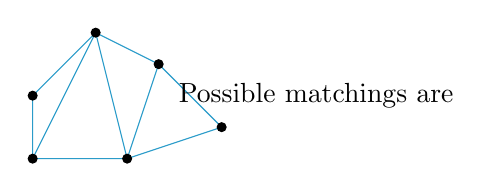
\begin{tikzpicture}[scale=0.8]
    % Graph Coordinates
    \coordinate (a) at (0,1);
    \coordinate (b) at (1,2);
    \coordinate (c) at (2,1.5);
    \coordinate (d) at (0,0);
    \coordinate (e) at (1.5,0);
    \coordinate (f) at (3,0.5);

    % Edges
    \draw[cyan!80!black] (a)--(b)--(c)--(f)--(e)--(d)--(a);
    \draw[cyan!80!black] (b)--(d);
    \draw[cyan!80!black] (b)--(e);
    \draw[cyan!80!black] (c)--(e);

    \foreach \p in {a,b,c,d,e,f} \filldraw (\p) circle (2pt);
    
    % Text
    \node at (4.5, 1) {Possible matchings are};
\end{tikzpicture}
\end{center}

\begin{center}
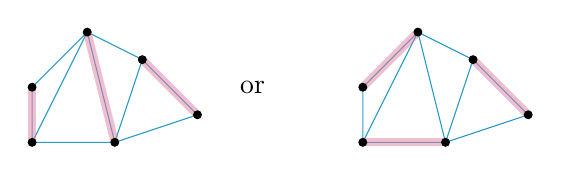
\begin{tikzpicture}[scale=0.7]
    % Matching 1 (Left)
    \begin{scope}[xshift=0cm]
        \coordinate (a) at (0,1); \coordinate (b) at (1,2);
        \coordinate (c) at (2,1.5); \coordinate (d) at (0,0);
        \coordinate (e) at (1.5,0); \coordinate (f) at (3,0.5);
        
        \draw[cyan!80!black] (a)--(b)--(c)--(f)--(e)--(d)--(a);
        \draw[cyan!80!black] (b)--(d); \draw[cyan!80!black] (b)--(e); \draw[cyan!80!black] (c)--(e);
        
        % Thick Matching Edges (Grey/Purple highlight style)
        \draw[line width=3pt, purple!50, opacity=0.5] (a)--(d);
        \draw[line width=3pt, purple!50, opacity=0.5] (b)--(e);
        \draw[line width=3pt, purple!50, opacity=0.5] (c)--(f);
        
        \foreach \p in {a,b,c,d,e,f} \filldraw (\p) circle (2pt);
    \end{scope}

    \node at (4, 1) {or};

    % Matching 2 (Right)
    \begin{scope}[xshift=6cm]
        \coordinate (a) at (0,1); \coordinate (b) at (1,2);
        \coordinate (c) at (2,1.5); \coordinate (d) at (0,0);
        \coordinate (e) at (1.5,0); \coordinate (f) at (3,0.5);
        
        \draw[cyan!80!black] (a)--(b)--(c)--(f)--(e)--(d)--(a);
        \draw[cyan!80!black] (b)--(d); \draw[cyan!80!black] (b)--(e); \draw[cyan!80!black] (c)--(e);
        
        % Thick Matching Edges
        \draw[line width=3pt, purple!50, opacity=0.5] (a)--(b);
        \draw[line width=3pt, purple!50, opacity=0.5] (d)--(e);
        \draw[line width=3pt, purple!50, opacity=0.5] (c)--(f);
        
        \foreach \p in {a,b,c,d,e,f} \filldraw (\p) circle (2pt);
    \end{scope}
\end{tikzpicture}
\end{center}
If we pair 2 with 5, 3 and 4 with 1, this is still a matching.
But we have 2 happy teams and can't form another one. It is not perfect...
\end{example}

Observation: The goal will be to pick a set of edges which do not share end vertices.

% 7.2 Definition
\begin{definition}
Let $G$ be any graph.
\begin{enumerate}
    \item[i)] A \textbf{\color{red}matching} for $G$ is a set $M \subseteq E(G)$ of pairwise disjoint edges.
    \item[ii)] $v \in V(G)$ is called \textbf{\color{red}$M$-saturated} if exists $e \in M$ s.t. $v \in e$ (i.e. if it is the endpoint of some edge in $M$). Otherwise, we call $v$ \textbf{\color{red}$M$-unsaturated}.
    \item[iii)] We call a matching $M$ \textbf{\color{red}maximal} iff $M \cup \{e\}$ is not a matching for any $e \in E(G) \setminus M$.
    \item[iv)] We say that $M$ is a \textbf{\color{red}maximum matching} if it has the largest cardinality among all possible matchings.
    \item[v)] Finally, we call $M$ \textbf{\color{red}perfect} if any $v \in V(G)$ is $M$-saturated.
\end{enumerate}
\end{definition}

% 7.3 Example
\begin{example}
Consider the graph $G = $
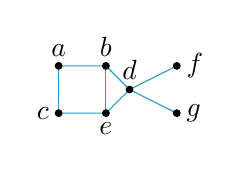
\begin{tikzpicture}[baseline=(current bounding box.center), scale=0.6]
    \coordinate (a) at (0,1); \coordinate (b) at (1,1);
    \coordinate (c) at (0,0); \coordinate (e) at (1,0);
    \coordinate (d) at (1.5, 0.5); \coordinate (f) at (2.5, 1);
    \coordinate (g) at (2.5, 0);

    \draw[cyan!80!black] (a)--(b)--(d)--(e)--(c)--(a);
    \draw[cyan!80!black] (b)--(e); \draw[cyan!80!black] (d)--(f); \draw[cyan!80!black] (d)--(g);

    \foreach \p in {a,b,c,d,e,f,g} \filldraw (\p) circle (2pt);
    
    \node[above] at (a) {$a$}; \node[above] at (b) {$b$}; \node[left] at (c) {$c$};
    \node[above] at (d) {$d$}; \node[below] at (e) {$e$}; \node[right] at (f) {$f$}; \node[right] at (g) {$g$};
\end{tikzpicture}.

Then
\begin{center}
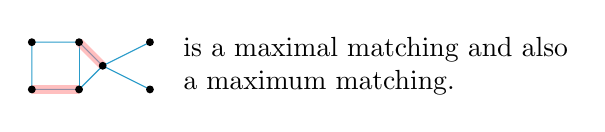
\begin{tikzpicture}[scale=0.6]
    % Graph 1
    \begin{scope}[xshift=0cm]
        \coordinate (a) at (0,1); \coordinate (b) at (1,1);
        \coordinate (c) at (0,0); \coordinate (e) at (1,0);
        \coordinate (d) at (1.5, 0.5); \coordinate (f) at (2.5, 1);
        \coordinate (g) at (2.5, 0);
        \draw[cyan!80!black] (a)--(b)--(d)--(e)--(c)--(a);
        \draw[cyan!80!black] (b)--(e); \draw[cyan!80!black] (d)--(f); \draw[cyan!80!black] (d)--(g);
        
        \draw[line width=3pt, red!50, opacity=0.5] (c)--(e);
        \draw[line width=3pt, red!50, opacity=0.5] (b)--(d);
        
        \foreach \p in {a,b,c,d,e,f,g} \filldraw (\p) circle (2pt);
    \end{scope}
    \node[right, align=left] at (3, 0.5) {is a maximal matching and also \\ a maximum matching.};
\end{tikzpicture}
\end{center}

Further,
\begin{center}
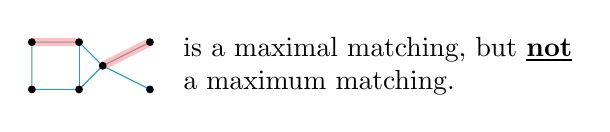
\begin{tikzpicture}[scale=0.6]
    % Graph 2
    \begin{scope}[xshift=0cm]
        \coordinate (a) at (0,1); \coordinate (b) at (1,1);
        \coordinate (c) at (0,0); \coordinate (e) at (1,0);
        \coordinate (d) at (1.5, 0.5); \coordinate (f) at (2.5, 1);
        \coordinate (g) at (2.5, 0);
        \draw[cyan!80!black] (a)--(b)--(d)--(e)--(c)--(a);
        \draw[cyan!80!black] (b)--(e); \draw[cyan!80!black] (d)--(f); \draw[cyan!80!black] (d)--(g);
        
        \draw[line width=3pt, red!50, opacity=0.5] (a)--(b);
        \draw[line width=3pt, red!50, opacity=0.5] (d)--(f);
        
        \foreach \p in {a,b,c,d,e,f,g} \filldraw (\p) circle (2pt);
    \end{scope}
    \node[right, align=left] at (3, 0.5) {is a maximal matching, but \textbf{\underline{not}} \\ a maximum matching.};
\end{tikzpicture}
\end{center}

Also,
\begin{center}
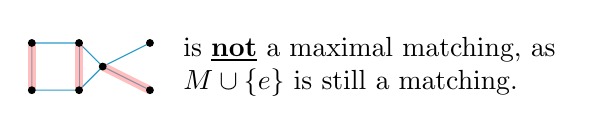
\begin{tikzpicture}[scale=0.6]
    % Graph 3
    \begin{scope}[xshift=0cm]
        \coordinate (a) at (0,1); \coordinate (b) at (1,1);
        \coordinate (c) at (0,0); \coordinate (e) at (1,0);
        \coordinate (d) at (1.5, 0.5); \coordinate (f) at (2.5, 1);
        \coordinate (g) at (2.5, 0);
        \draw[cyan!80!black] (a)--(b)--(d)--(e)--(c)--(a);
        \draw[cyan!80!black] (b)--(e); \draw[cyan!80!black] (d)--(f); \draw[cyan!80!black] (d)--(g);
        
        \draw[line width=3pt, red!50, opacity=0.5] (a)--(c);
        \draw[line width=3pt, red!50, opacity=0.5] (b)--(e);
        \draw[line width=3pt, red!50, opacity=0.5] (d)--(g);
        
        \foreach \p in {a,b,c,d,e,f,g} \filldraw (\p) circle (2pt);
    \end{scope}
    \node[right, align=left] at (3, 0.5) {is \textbf{\underline{not}} a maximal matching, as \\ $M \cup \{e\}$ is still a matching.};
\end{tikzpicture}
\end{center}

Finally, there are no perfect matchings as $|V(G)|$ is odd.
\end{example}

% 7.4 Remark
\begin{remark}
\begin{enumerate}
    \item[1)] Any perfect matching is a maximum matching.
    \item[2)] Any maximum matching is maximal.
    \item[3)] If $G$ has a perfect matching, then $|G|$ is even.
\end{enumerate}
Further, any matching $M$ is perfect iff it is a maximum matching iff $|M| = \frac{|V|}{2}$.
\end{remark}

% 7.5 Examples
\begin{example}
\begin{center}
\begin{tabular}{c c c c}
Graph $G$ & maximal & maximum & perfect \\[0.5em]
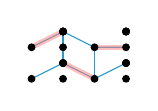
\begin{tikzpicture}[scale=0.4, baseline=-0.5ex]
    \draw[cyan!80!black] (0,0)--(1,0.5)--(2,0)--(3,0);
    \draw[cyan!80!black] (0,-1)--(1,-0.5)--(2,-1)--(3,-0.5);
    \draw[cyan!80!black] (1,0.5)--(1,-0.5); \draw[cyan!80!black] (2,0)--(2,-1);
    \draw[line width=2pt, red!50, opacity=0.5] (0,0)--(1,0.5);
    \draw[line width=2pt, red!50, opacity=0.5] (2,0)--(3,0);
    \draw[line width=2pt, red!50, opacity=0.5] (1,-0.5)--(2,-1);
    \foreach \x in {0,1,2,3} { \filldraw (\x,0) circle (3pt); \filldraw (\x,-1) circle (3pt); \filldraw (1,0.5) circle (3pt); \filldraw (1,-0.5) circle (3pt); \filldraw (3,0.5) circle (3pt); \filldraw (3,-0.5) circle (3pt); } 
    % Note: Simplified sketch for the table
\end{tikzpicture} & \textbf{\color{green!60!black}\checkmark} & \textbf{\color{red}X} & \textbf{\color{red}X} \\
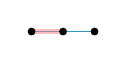
\begin{tikzpicture}[scale=0.4, baseline=-0.5ex]
    % Another matching on same graph
    \draw[cyan!80!black] (0,0)--(1,0)--(2,0);
    \draw[line width=2pt, red!50, opacity=0.5] (0,0)--(1,0);
    \filldraw (0,0) circle (3pt); \filldraw (1,0) circle (3pt); \filldraw (2,0) circle (3pt);
\end{tikzpicture} & \textbf{\color{green!60!black}\checkmark} & \textbf{\color{green!60!black}\checkmark} & \textbf{\color{red}X} \\
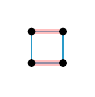
\begin{tikzpicture}[scale=0.4, baseline=-0.5ex]
    % Perfect matching example
    \draw[cyan!80!black] (0,0)--(1,0)--(1,1)--(0,1)--(0,0);
    \draw[line width=2pt, red!50, opacity=0.5] (0,0)--(1,0);
    \draw[line width=2pt, red!50, opacity=0.5] (0,1)--(1,1);
    \foreach \x in {0,1} \foreach \y in {0,1} \filldraw (\x,\y) circle (3pt);
\end{tikzpicture} & \textbf{\color{green!60!black}\checkmark} & \textbf{\color{green!60!black}\checkmark} & \textbf{\color{green!60!black}\checkmark} 
\end{tabular}
\end{center}
Note that there can't be a perfect matching, even though $|G|=10$ is even, as any matching uses at most one of $hg, ig$ and $jg$.

We see that while it is rather easy to decide whether a matching is maximal or perfect, things are less clear for a maximum matching. Our next goal is to develop a criterion to help us decide that, called Berge's Theorem.
\end{example}

% 7.6 Definition
\begin{definition}
Let $G$ be a graph and $M$ a matching for $G$ and $p$ a path in $G$.
\begin{enumerate}
    \item[1)] We say that $p$ is \textbf{\color{red}$M$-alternating} if its edges alternate between edges inside and outside $M$.
    \item[2)] We call $p$ \textbf{\color{red}$M$-augmenting} if it is $M$-alternating and its start and end vertex are distinct and both \underline{not} $M$-saturated.
\end{enumerate}
\end{definition}

How does this relate to maximum matchings?

% 7.7 Example
\begin{example}
Consider the graph $G$ with matching $M$ below.
\begin{center}
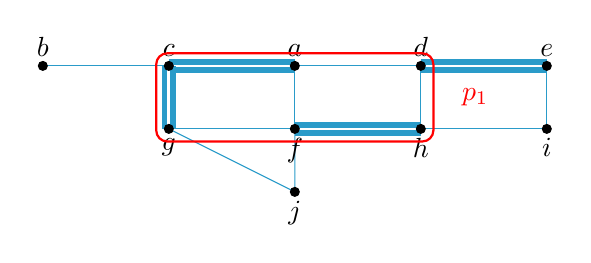
\begin{tikzpicture}[scale=0.8]
    \coordinate (b) at (0,1); \coordinate (c) at (2,1); \coordinate (a) at (4,1); \coordinate (d) at (6,1);
    \coordinate (g) at (2,0); \coordinate (f) at (4,0); \coordinate (h) at (6,0);
    \coordinate (e) at (8,1); \coordinate (i) at (8,0); \coordinate (j) at (4,-1);

    % Box structure
    \draw[cyan!80!black] (b)--(c); 
    \draw[cyan!80!black, line width=2pt, double, double distance=1pt] (c)--(a); % Matching
    \draw[cyan!80!black] (a)--(d);
    \draw[cyan!80!black, line width=2pt, double, double distance=1pt] (d)--(e); % Matching
    
    \draw[cyan!80!black, line width=2pt, double, double distance=1pt] (c)--(g); % Matching
    \draw[cyan!80!black] (a)--(f);
    \draw[cyan!80!black] (d)--(h);
    \draw[cyan!80!black] (e)--(i);
    
    \draw[cyan!80!black] (g)--(f);
    \draw[cyan!80!black, line width=2pt, double, double distance=1pt] (f)--(h); % Matching
    \draw[cyan!80!black] (h)--(i);
    
    \draw[cyan!80!black] (g)--(j)--(f);
    
    \foreach \p in {a,b,c,d,e,f,g,h,i,j} \filldraw (\p) circle (2pt);
    
    \node[above] at (b) {$b$}; \node[above] at (c) {$c$}; \node[above] at (a) {$a$}; \node[above] at (d) {$d$}; \node[above] at (e) {$e$};
    \node[below] at (g) {$g$}; \node[below] at (f) {$f$}; \node[below] at (h) {$h$}; \node[below] at (i) {$i$}; \node[below] at (j) {$j$};
    
    % Red Path Highlight
    \draw[red, thick, rounded corners] (1.8,-0.2) rectangle (6.2, 1.2);
    \node[right, red] at (6.5, 0.5) {$p_1$};
\end{tikzpicture}
\end{center}
The path $p_1 = (g, c, a, d, e, i, h, j)$ is $M$-alternating, but not $M$-augmenting, its start vertex $g$ is $M$-saturated.

On the other hand, the path $p_2 = (b, c, a, d, e, i, h, j)$ is $M$-augmenting. In particular, it is $M$-alternating. What happens if we define a new edge set $M'$ by containing all edges of $M$ outside of $p$ and also exactly those edges of $p$ which were not in $M$?

For $p_1=(g,c,a,d,e,i,h,j)$ which was $M$-alternating, but not $M$-augmenting, we obtain an edge set which is \underline{not} a matching.
For the $M$-augmenting path $p_2=(b,c,a,d,e,i,h,j)$, on the other hand, the set $M'$ is indeed a matching. Moreover, it contains more edges than $M$.
Hence, $M$ was not a maximum matching for $G$.
\end{example}

% 7.8 Theorem
\begin{theorem}
Let $G$ be a graph and $M$ a matching for $G$. Then $M$ is a maximum matching iff there is \underline{no} $M$-augmenting path in $G$.
\end{theorem}

\begin{proof}
``$\Rightarrow$'' We proceed by contraposition. Assume $M$ is a matching and $p=(x_1, \dots, x_n)$ an $M$-augmenting path. We will show that $M$ is not maximal. If the edges of $p$ are $e_1, e_2, \dots, e_{n-1}$, then as $x_1$ is not $M$-saturated, we get that $e_1 \notin M$. As $p$ is $M$-alternating also $e_3, e_5, \dots$, i.e. all odd numbered edges are not in $M$, while all even numbered edges are in $M$. As also $x_n$ is not $M$-saturated, $e_{n-1} \notin M$, whence $n-1$ is odd and $n$ is even. Now define
\[ M' := M \setminus \{e_2, e_4, \dots, e_{n-2}\} \cup \{e_1, e_3, \dots, e_{n-3}, e_{n-1}\}. \]
Note that $|M'| = |M| + 1$. We claim that $M'$ is a matching, proving that $M$ was not a maximum. But this is clear, as through the change of edges only $x_1$ and $x_n$ are newly $M'$-saturated. As they were not $M$-saturated, $x_1$ is only the endpoint of $e_1$ in $M'$ and $x_n$ only of $e_{n-1}$ in $M'$. Hence $M'$ is again a matching, larger than $M$.

``$\Leftarrow$'' We proceed again by contraposition. Assume $M$ is a matching of $G$ which is not a maximum, i.e. there is another matching $M'$ of $G$ with $|M'| > |M|$. We aim to find an $M$-augmenting path in $G$.
To this end, we define a subgraph $H \subseteq G$ via $V(H)=V(G)$ and $E(H) = M' \Delta M (= M' \setminus M \cup M \setminus M')$.
\begin{itemize}
    \item Note that $|M' \setminus M| = |M'| - |M' \cap M| > |M| - |M' \cap M| = |M \setminus M'|$, whence $H$ contains strictly more edges from $M'$ than from $M$.
    \item Further, $\Delta(H) \le 2$. To see that, consider $x \in V(H)$ arbitrary. Then there can be at most one edge from $M$ containing $x$ and also at most one other edge from $M'$, as $M$ and $M'$ are matchings. Hence $\delta(x) \le 2$, as desired.
    \item Now we know that every connected component of $H$ either is a cycle of even length (using the same number of edges from $M$ and $M'$), or a path. As $|M' \setminus M| > |M \setminus M'|$, there must be at least one connected component in $H$ which is a path of odd length, starting and ending with an edge in $M'$. This yields the desired $M$-augmenting path in $G$. \qedhere
\end{itemize}
\end{proof}

\section{Hall's Marriage Theorem}

Finding matchings becomes of special interest in bipartite graphs. Historically, the questions were visualised by trying to match couples for marriage. As this does not actually give a bipartite graph, we will put ourselves into the holiday spirit and will discuss bipartite graphs, where one part represents a set of children and the other part a set of presents. We will try to help Santa and develop a criterion to decide whether we can make all the children happy.

% 7.9 Example
\begin{example}
Consider the bipartite graphs below with $V(G)=X \cup Y$, where $X$ represents a set of children and $Y$ a set of presents.
\begin{center}
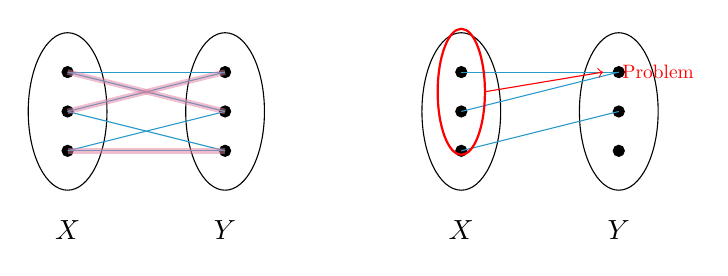
\begin{tikzpicture}[scale=1]
    % Case 1
    \begin{scope}[xshift=0cm]
        % X nodes (children)
        \draw (0,0) ellipse (0.5 and 1); \node at (0,-1.5) {$X$};
        \coordinate (x1) at (0, 0.5); \coordinate (x2) at (0, 0); \coordinate (x3) at (0, -0.5);
        
        % Y nodes (presents)
        \draw (2,0) ellipse (0.5 and 1); \node at (2,-1.5) {$Y$};
        \coordinate (y1) at (2, 0.5); \coordinate (y2) at (2, 0); \coordinate (y3) at (2, -0.5);
        
        \foreach \p in {x1,x2,x3,y1,y2,y3} \filldraw (\p) circle (2pt);
        
        % Edges
        \draw[cyan!80!black] (x1)--(y1); \draw[cyan!80!black] (x1)--(y2);
        \draw[cyan!80!black] (x2)--(y1); \draw[cyan!80!black] (x2)--(y3);
        \draw[cyan!80!black] (x3)--(y2); \draw[cyan!80!black] (x3)--(y3);
        
        % Matching highlights
        \draw[line width=2pt, purple!50, opacity=0.5] (x1)--(y2);
        \draw[line width=2pt, purple!50, opacity=0.5] (x2)--(y1);
        \draw[line width=2pt, purple!50, opacity=0.5] (x3)--(y3);
    \end{scope}
    
    % Case 2
    \begin{scope}[xshift=5cm]
        \draw (0,0) ellipse (0.5 and 1); \node at (0,-1.5) {$X$};
        \coordinate (x1) at (0, 0.5); \coordinate (x2) at (0, 0); \coordinate (x3) at (0, -0.5);
        
        \draw (2,0) ellipse (0.5 and 1); \node at (2,-1.5) {$Y$};
        \coordinate (y1) at (2, 0.5); \coordinate (y2) at (2, 0); \coordinate (y3) at (2, -0.5);
        
        \foreach \p in {x1,x2,x3,y1,y2,y3} \filldraw (\p) circle (2pt);
        
        % Edges
        \draw[cyan!80!black] (x1)--(y1); 
        \draw[cyan!80!black] (x2)--(y1); 
        \draw[cyan!80!black] (x3)--(y2); 
        
        % Problem circle
        \draw[red, thick] (0, 0.25) ellipse (0.3 and 0.8);
        \draw[red, ->] (0.3, 0.25) -- (1.8, 0.5);
        \node[red, scale=0.7] at (2.5, 0.5) {Problem};
    \end{scope}
\end{tikzpicture}
\end{center}
$\to$ There is a matching which makes all children happy. \\
$\to$ There are two children which both only want the first present. Hence, there is no appropriate matching.

How can we know from the graph when an appropriate matching exists? This is solved in Philip Hall's marriage theorem.
\end{example}

% 7.10 Definition
\begin{definition}
Let $G$ be a bipartite graph with parts $X$ and $Y$. We say that $X$ is \textbf{\color{red}matched into} $Y$ if there is a matching $M$ for $G$ s.t. every $x \in X$ is $M$-saturated.
\end{definition}

% 7.11 Remark
\begin{remark}
As above, $X$ is matched into $Y$ iff there is an injective function $f: X \to Y$ s.t. $\{x, f(x)\} \in E(G)$ for all $x \in X$.
\end{remark}

% 7.12 Theorem
\begin{theorem}
Let $G$ be a bipartite graph with parts $X$ and $Y$. Then $X$ is matched into $Y$ iff for all sets $S \subseteq X$ we have $|S| \le |N(S)|$.
\end{theorem}

\begin{proof}
``$\Rightarrow$'' Assume $X$ is matched into $Y$, say via $f: X \to Y$. Let $S \subseteq X$ be arbitrary. As $\{x, f(x)\} \in E(G)$ for all $x \in X$, we actually get that $f(S) \subseteq N(S)$. As further $f$ is injective, by definition we get that $|S| \le |N(S)|$, as desired.

``$\Leftarrow$'' Assume now that for any $S \subseteq X$ we have $|S| \le |N(S)|$.
We want to show that there is a matching $M$ which matches $X$ into $Y$. Let $M$ be any maximum matching. We claim that $M$ matches $X$ into $Y$.
Aiming for a contradiction, assume not, i.e. there is some $u \in X$ which is not $M$-saturated. Define the set
\[ A := \{ v \in V(G) \mid \text{exists an } M\text{-alternating } uv\text{-path} \}. \]
We claim that $S := A \cap X$ violates the assumption, i.e. $|S| > |N(S)|$.
We will split the proof int 2 parts. Let $T := A \cap Y$.
Let's start with some observations.
First note that as $u$ is \underline{not} $M$-saturated, for any $M$-alternating path $p=(u=u_1, u_2, \dots, u_k)$ we have
\[ u_i u_{i+1} \in M \text{ iff } i \in 2\mathbb{Z} \text{ iff } u_i \in T \text{ iff } u_{i+1} \in S. \]
Further, as $M$ is maximal there are no $M$-augmenting paths. In particular, any $v \in A \setminus \{u\}$ must be $M$-saturated.

\underline{Claim 1: $|S|-1 = |T|$.}
We define a function $f: S \setminus \{u\} \to T$ via the following:
If $x \in S \setminus \{u\}$ then ex. $p_x = (u=u_1, u_2, \dots, u_k=x)$ $M$-alternating. Then as $x \in S$, $u_{k-1} u_k \in M$ and $M$ is a matching, $u_{k-1}$ is the only neighbour of $x$ s.t. $u_{k-1} x \in M$. Further $u_{k-1} \in T$ and we set $f(x) := u_{k-1}$. As $M$ is a matching, $f$ is injective. Further, for any $y \in T$ by definition there is an $M$-alternating $uy$-path $p_y = (u=y_1, y_2, \dots, y_\ell=y)$. As $y \in Y$, $y_{\ell-1}y \notin M$ and $y_\ell$ is $M$-saturated, there must be a vertex $x \in X$ s.t. $y_\ell x \in M$. But then $p_y^{-1}(x) = (u, y_1, \dots, y_\ell=y, x)$ is an $M$-alternating path whence $x \in S$. By definition of $f$, we get that $f(x)=y$, whence $y \in \text{range}(f)$. Thus, $f$ is a bijection and $|S \setminus \{u\}| = |S|-1 = |T|$.

\underline{Claim 2: $N(S)=T$.}
``$\supseteq$'' Let $w \in N(S)$, i.e. exists $s \in S$ s.t. $sw \in E(G)$. As $s \in S \subseteq X$, the vertex $w$ must be in $Y$. Further, let $p_s$ be an $M$-alternating $us$-path. Then by adjoining $w$ to $p_s$, we obtain an $M$-alternating $uw$-path, whence $w \in T$, as desired.
``$\subseteq$'' Let $w \in T$ be arbitrary and $s := f^{-1}(t)$ with $f$ defined as in Claim 1. Then $s \in S \setminus \{u\}$ and $w \in N(s)$, as desired.

Conclusively, we have constructed a set $S \subseteq X$ s.t.
\[ |S| = |T|+1 = |N(S)|+1 > |N(S)|, \]
contradicting our assumptions.
Thus, such a vertex $u$ cannot exist, whence all vertices in $X$ are $M$-saturated and $M$ matches $X$ into $Y$. \qedhere
\end{proof}

\topic{Application - System of Representatives}

% 7.13 Definition
\begin{definition}
Let $\mathcal{F} = \{S_1, S_2, \dots, S_k\}$ be a family of non-empty sets.
A \textbf{\color{red}system of distinct representatives} for $\mathcal{F}$ is a set $\{x_1, x_2, \dots, x_k\}$ s.t. $x_i \in S_i$ and the $x_i$ are pairwise distinct.
\end{definition}

% 7.14 Example
\begin{example}
Let $S_1=\{2,8\}, S_2=\{8\}, S_3=\{5,7\}, S_4=\{2,4,8\}, S_5=\{2,4\}$.
Can we find a system of representatives for $\mathcal{F}=\{S_1, \dots, S_5\}$?
Let's visualise the problem:

\begin{center}
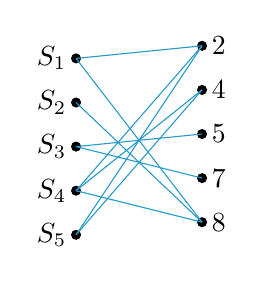
\begin{tikzpicture}[scale=0.8]
    % Sets
    \foreach \i in {1,...,5} \coordinate (s\i) at (0, 3 - 0.7*\i);
    \node[left] at (s1) {$S_1$}; \node[left] at (s2) {$S_2$}; \node[left] at (s3) {$S_3$};
    \node[left] at (s4) {$S_4$}; \node[left] at (s5) {$S_5$};
    \foreach \i in {1,...,5} \filldraw (s\i) circle (2pt);
    
    % Elements
    \coordinate (e2) at (2, 2.5); \node[right] at (e2) {2};
    \coordinate (e4) at (2, 1.8); \node[right] at (e4) {4};
    \coordinate (e5) at (2, 1.1); \node[right] at (e5) {5};
    \coordinate (e7) at (2, 0.4); \node[right] at (e7) {7};
    \coordinate (e8) at (2, -0.3); \node[right] at (e8) {8};
    \foreach \e in {e2,e4,e5,e7,e8} \filldraw (\e) circle (2pt);
    
    % Edges based on containment
    \draw[cyan!80!black] (s1)--(e2); \draw[cyan!80!black] (s1)--(e8);
    \draw[cyan!80!black] (s2)--(e8);
    \draw[cyan!80!black] (s3)--(e5); \draw[cyan!80!black] (s3)--(e7);
    \draw[cyan!80!black] (s4)--(e2); \draw[cyan!80!black] (s4)--(e4); \draw[cyan!80!black] (s4)--(e8);
    \draw[cyan!80!black] (s5)--(e2); \draw[cyan!80!black] (s5)--(e4);
\end{tikzpicture}
\end{center}
With this visualisation the question translates into asking whether $\mathcal{F}$ is matched into $U = \cup S_i$.
Let $S = \{S_1, S_2, S_4, S_5\}$. Then $|S|=4$. On the other hand, $|N(S)| = |\{2,4,8\}| = 3$. So $|S| > |N(S)|$ and by Hall's marriage theorem, there is no system of distinct representatives for $\mathcal{F}$. If we consider $\mathcal{F}_0 := \{S_1, S_2, S_3, S_4\}$ however, then a system of distinct representatives is given by $\{2,8,5,4\}$.
\end{example}

% 7.15 Theorem
\begin{theorem}
Let $\mathcal{F}=\{S_1, S_2, \dots, S_k\}$ be a family of nonempty sets. Then $\mathcal{F}$ has a system of representatives iff for any $I \subseteq \{1, 2, \dots, k\}$ we have that $|I| \le |\cup_{i \in I} S_i|$.
\end{theorem}

\begin{proof}
Exercise, easy consequence from Hall's marriage theorem.
\end{proof}

\section{The K\"{o}nig-Egerv\'{a}ry Theorem}
We want to finish the chapter on matchings by relating them to yet another very important graph concept - the one of vertex covers.

% 7.16 Definition
\begin{definition}
Let $G$ be a graph. A \textbf{\color{red}vertex cover} for $G$ is a vertex set $C \subseteq V(G)$ s.t. every edge of $G$ has at least one endvertex in $C$, i.e. $\forall e \in E(G) \exists x \in C \text{ s.t. } x \in e$.
A vertex cover is called a \textbf{\color{red}minimum vertex cover} if there is no vertex cover of smaller cardinality.
\end{definition}

% 7.17 Application
\topic{Application}
Imagine a museum with many galleries. We want to position guards within the galleries that have all art pieces in sight. If we model galleries as edges and places where at least two galleries meet as vertices, then we obtain a graph. Now every vertex cover for $G$ would provide an appropriate list of locations to place our guards. Of course, we want to minimize our spendings when usually we are interested in finding a minimum vertex cover.

% 7.18 Remark
\begin{remark}
\begin{enumerate}
    \item[1)] Every graph $G$ has a vertex cover, namely $V_G$.
    \item[2)] If $C$ is a vertex cover for $G$ and $C \subseteq D$, then $D$ is a vertex cover for $G$.
\end{enumerate}
\end{remark}

% 7.19 Example
\begin{example}
Consider $G$ given by
\begin{center}
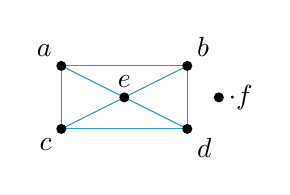
\begin{tikzpicture}[scale=0.8]
    \coordinate (c) at (0,0); \coordinate (d) at (2,0);
    \coordinate (a) at (0,1); \coordinate (b) at (2,1);
    \coordinate (e) at (1, 0.5);
    
    \draw[cyan!80!black] (a)--(b)--(d)--(c)--(a);
    \draw[cyan!80!black] (a)--(e); \draw[cyan!80!black] (b)--(e); \draw[cyan!80!black] (c)--(e); \draw[cyan!80!black] (d)--(e);
    
    \foreach \p in {a,b,c,d,e} \filldraw (\p) circle (2pt);
    
    \node[above left] at (a) {$a$}; \node[above right] at (b) {$b$};
    \node[below left] at (c) {$c$}; \node[below right] at (d) {$d$};
    \node[above] at (e) {$e$};
    \node[right] at (2.5, 0.5) {$\cdot f$};
    \filldraw (2.5, 0.5) circle (2pt);
\end{tikzpicture}
\end{center}
Then one vertex cover is given by $C_1 := \{a,b,c,d\}$. But also, $C_2 := \{a,e,d\}$ is a vertex cover of smaller cardinality. It is not hard to see that there is no vertex cover containing only two vertices, whence $C_2$ is minimal.
\end{example}

For each of the graphs below, find a maximum matching $M$ and a minimum vertex cover $C$. Can you conjecture a relation between $|M|$ and $|C|$ for arbitrary graphs $G$?

\begin{center}
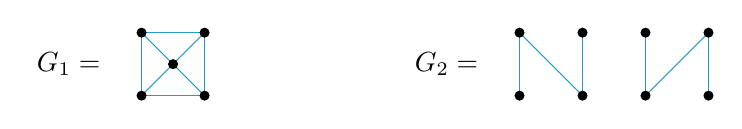
\begin{tikzpicture}[scale=0.8]
    % G1 (Square with center point)
    \begin{scope}[xshift=0cm]
        \coordinate (a) at (0,1); \coordinate (b) at (1,1);
        \coordinate (c) at (0,0); \coordinate (d) at (1,0);
        \coordinate (f) at (0.5, 0.5);
        \draw[cyan!80!black] (a)--(b)--(d)--(c)--(a);
        \draw[cyan!80!black] (a)--(f); \draw[cyan!80!black] (b)--(f);
        \draw[cyan!80!black] (c)--(f); \draw[cyan!80!black] (d)--(f);
        \foreach \p in {a,b,c,d,f} \filldraw (\p) circle (2pt);
        \node[left] at (-0.5, 0.5) {$G_1=$};
    \end{scope}

    % G2 (Bipartite graph)
    \begin{scope}[xshift=5cm]
        \foreach \i in {1,2,3,4} \coordinate (u\i) at (\i, 0);
        \coordinate (v1) at (1,1); \coordinate (v2) at (2,1); \coordinate (v3) at (3,1); \coordinate (v4) at (4,1);
        \draw[cyan!80!black] (v1)--(u1); \draw[cyan!80!black] (v2)--(u2); \draw[cyan!80!black] (v3)--(u3); \draw[cyan!80!black] (v4)--(u4);
        \draw[cyan!80!black] (v1)--(u2); \draw[cyan!80!black] (v4)--(u3);
        \foreach \p in {u1,u2,u3,u4,v1,v2,v3,v4} \filldraw (\p) circle (2pt);
        \node[left] at (0.5, 0.5) {$G_2=$};
    \end{scope}
\end{tikzpicture}
\end{center}
We see that in $G_1$, $|M|=3 < 4 = |C|$, while in $G_2$, $|M|=3 < |C|$ (Wait, notes say $|M|=3=|C|$ for G2).
What is the difference in both graphs? We note that $G$ is bipartite.

% 7.20 Lemma
\begin{lemma}
Let $G$ be a graph, $M$ any matching for $G$ and $C$ any vertex cover for $G$. Then $|M| \le |C|$. In particular, a maximum matching contains at most as many edges as a minimal vertex cover contains vertices.
\end{lemma}

\begin{proof}
Let $M$ be any matching for $G$, say $M=\{e_1, e_2, \dots, e_k\}$, and $C$ any vertex cover. For any $e_i \in M$ there is a vertex $x_i \in C$ incident with $e_i$. As all $e_i$'s are disjoint, all the $x_1, x_2, \dots, x_k$ are distinct. Thus, $C$ contains at least as many elements as $M$, i.e. $|M| \le |C|$. \qedhere
\end{proof}

Now, what changes if we restrict ourselves to bipartite graphs? Somehow we have more control over the relation between vertices and edges. Indeed, the Hungarian mathematicians D\'{e}nes K\"{o}nig and Jen\H{o} Egerv\'{a}ry independently discovered the following in 1931.

% 7.21 Theorem (Konig-Egervary)
\begin{theorem}
Let $G$ be a bipartite graph. Then any maximum matching has the same cardinality as any minimum vertex cover.
\end{theorem}

\begin{proof}
Consider an arbitrary bipartite graph $G$ and a maximum matching $M$. We will show that there exists a vertex cover $C$ s.t. $|M|=|C|$. By Lemma 7.20, $C$ then is a minimum vertex cover. Let $X$ and $Y$ form a bipartition of $V_G$.
If every $x \in X$ is $M$-saturated, then $|X|=|M|$. Clearly, as $G$ is bipartite, the set $C:=X$ is a vertex cover for $G$, whence $|C|=|X|=|M|$ is as desired.
Now, assume \underline{not} every $x \in X$ is $M$ saturated.
Let $U := \{x \in X \mid x \text{ is not } M\text{-saturated}\}$. Then $|M|+|U| = |X|$. (*)
Similar to Hall's Lemma, set
$A := \{ v \in V(G) \mid \text{ex. an } M\text{-alternating } uv\text{-path for some } u \in U \}$.
Further, set $S := A \cap X$ and $T := A \cap Y$. We claim that $C := (X \setminus S) \cup UT$ is a vertex cover with $|C|=|M|$.
Exactly as in the proof of 7.12, we can show that
1) Every vertex in $(S \setminus U) \cup T$ is $M$-saturated.
2) $|S \setminus U| = |T|$.
3) $T = N(S)$.

Thus, we immediately get that $|T| = |S| - |U|$ (**) and thus
\[ |C| = |X \setminus S| \cup |T| = |X| \setminus |S| + |T| \overset{(**)}{=} |X| - |S| + |S| - |U| = |X| - |U| \overset{(*)}{=} |M|, \text{ as desired.} \]
It remains to show that $C$ is a vertex cover for $G$.
To this end, let $e=xy$ be an arbitrary edge with $x \in X, y \in Y$. We need to show that at least one of $x$ or $y$ is in $C=(X \setminus S) \cup T$.
If $x \notin S$, i.e. $x \in X \setminus S$, we are done. Otherwise $x \in S$, whence $y \in N(S) = T$, as desired. This finishes the proof. \qedhere
\end{proof}